\documentclass[]{tukediphc}
%% -----------------------------------------------------------------
%% tento subor ma kodovanie utf-8
%%
%% na kompilaciu pouzivajte format pdfcslatex 
%%
%% vytvorene distribuciou texlive 2009-7, OS GNU/Linux
%% vytvorene distribuciou TeXLive 2010, OS Win XP
%% februar 2013
%% -----------------------------------------------------------------
\usepackage[utf8]{inputenc}
%\usepackage[T1]{fontenc}
\usepackage{lmodern,textcase}
\usepackage[slovak]{babel}\renewcommand{\figurename}{Obr\'azok}
\def\refname{Zoznam pou\v{z}itej literat\'ury}
\usepackage{latexsym}
\usepackage{dcolumn} % zarovnanie cisiel v tabulke podla des. ciarky
\usepackage{hhline}
\usepackage{amsmath}
\usepackage{subfig}
\usepackage{nicefrac} % pekne zlomky
\usepackage{upgreek} % napr. $\upmu\mathrm{m}$ pre mikrometer ...
\usepackage[final]{showkeys}%color%notref%notcite%final
\usepackage[slovak,noprefix]{nomencl}
\makeglossary % prikaz na vytvorenie suboru .glo
\usepackage{parskip}% 'zhusti' polozky obsahu
%%
%\usepackage[dvips]{graphicx}
%\DeclareGraphicsExtensions{.eps}
\usepackage[pdftex]{graphicx}
\DeclareGraphicsExtensions{.pdf,.png,.jpg,.mps}
\graphicspath{{figures/}} % priecinok na obrazky
%%
%% Cislovane citovanie
%\usepackage[numbers]{natbib}
%%
%% Citovanie podľa mena autora a roku
\usepackage{natbib} %\citestyle{chicago}
% -----------------------------------------------------------------
%% tlač !!!
\usepackage[pdftex,unicode=true,bookmarksnumbered=true,
bookmarksopen=true,pdfmenubar=true,pdfview=Fit,linktocpage=true,
pageanchor=true,bookmarkstype=toc,pdfpagemode=UseOutlines,
pdfstartpage=1]{hyperref}
\hypersetup{%
baseurl={http://www.tuke.sk/sevcovic},
pdfcreator={pdfcsLaTeX},
pdfkeywords={Riadenie procesov, Oceliarstvo, Vizualizácia, Virtuálna realita, Matematické modelovanie},
pdftitle={Písomná príprava k predmetu Informačné technológie v riadení procesov},
pdfauthor={Michal Takáč},
pdfsubject={Dizertačná skúška}
} 
%% nehodiace zakomentujte !
%\dippraca{Elaborát z predmetu Riadenie procesov}
%\bakpraca{Príprava na dizertačnú skúšku}
%%
\nazov{Písomná príprava k predmetu Informačné technológie v riadení procesov}
%% ked praca nema 'podnazov' zakomentujte nasledujuci riadok
%% alebo polozku nechajte prazdnu
\podnazov{}
\autor{Ing.~Michal Takáč}
\veduciprace{doc.~Ing.~Ján~Kačur, PhD.}
\univerzita{Technická univerzita v~Košiciach}
\fakulta{Fakulta baníctva, ekológie, riadenia a geotechnológií}
\skratkafakulty{FBERG}
\katedra{Ústav riadenia a informatizácie výrobných procesov}
\skratkakatedry{URIVP}
\odbor{Riadenie procesov}
\specializacia{Kybernetika}
\abstrakt{Abstrakt je povinnou súčasťou každej práce. Je výstižnou
charakteristikou obsahu dokumentu. Nevyjadruje hodnotiace stanovisko
autora. Má byť\/ taký informatívny, ako to povoľuje podstata práce.
Text abstraktu sa píše ako jeden odstavec. Abstrakt neobsahuje odkazy
na samotný text práce. Mal by mať\/ rozsah 250 až 500 slov. Pri
štylizácii sa používajú celé vety, slovesá v činnom rode a tretej
osobe. Používa sa odborná terminológia, menej zvyčajné termíny,
skratky a~symboly sa pri prvom výskyte v texte definujú.}
\klucoveslova{Riadenie procesov, Oceliarstvo, Vizualizácia, Virtuálna realita, Matematické modelovanie}
\datumodovzdania{29. 5. 2020}
\mesto{Košice}

\begin{document}
\renewcommand\theHfigure{\theHsection.\arabic{figure}}
\renewcommand\theHtable{\theHsection.\arabic{table}}
\bibliographystyle{dcu}

\prvastrana


\thispagestyle{empty}
\tableofcontents
\newpage
%
%\thispagestyle{empty}
%%\addcontentsline{toc}{section}{\numberline{}Zoznam obrázkov}
%\listoffigures
%\newpage
%
%\thispagestyle{empty}
%%\addcontentsline{toc}{section}{\numberline{}Zoznam tabuliek}
%\listoftables
%\newpage

%%%%%%%%%%%%%%%%%%%%%%%%%%%%%%%%%

\setcounter{page}{1}
\setcounter{equation}{0}
\setcounter{figure}{0}
\setcounter{table}{0}

\section{Úvod}

%elaborát (písomná príprava) môže byť v rozsahu 10-15 strán. Nakoľko predmet má názov "Informačne technológie v riadení procesov" môžete použiť podklady z minimovky ale spomeňte v príprave aj SCADA/HMI systémy a ich možností (t.j. prepojenie človek-proces, vizualizácia dát) a stručne aj komunikačných protokolov (najmä OPC, alebo iných nakoľko predpokladám, že Vás model má ambíciu byť aplikovaný aj online), ďalej data processing (do modelu musia byť dáta vhodne upravené/spracované, napr. v Matlabe), a trochu aj management IS (možno to čo navrhujete Vy v 3D pohľade poslúži pre rozhodovanie vyššiemu managementu spolu s nejakou SCADOU a predikčným modelom (môžte vymenovať aké sa používajú) ako optimálne riadiť konvertorový proces). Pretože informačný systém to sú technológie monitorovania, analýzy, spracovania a uchovania a distribúcie dát pre ich ďalšie využitie.

Informačné systémy v procesnom riadení sú implementované pre rôzne škály riadiacich systémov, ktorých môže tvoriť niekoľko modulárnych panelových automatov až po veľké, vzájomne prepojené a interaktívne distribuované riadiace systémy s mnohými tisíckami prevádzkových pripojení.

Najjednoduchšie riadiace systémy sú založené na malých diskrétnych regulátoroch, z ktorých každý má jednu regulačnú slučku. Zvyčajne sú namontované na panel, ktorý umožňuje priame odčítanie hodnôt z predného panela a poskytuje prostriedky na manuálny zásah operátora, a to buď na manuálne riadenie procesu, alebo na zmenu požadovaných riadiacich hodnôt.


Pre ložitejšie zariadenia PCS sú robotické a vykonávajú veľa úloh. Zariadenia PCS môžu komunikovať svoje údaje s počítačovou aplikáciou podnikového plánovania podnikových zdrojov (ERP) prostredníctvom softvéru middleware nazývaného systém vykonávania výroby (MES).

Cieľom riadenia procesu je udržiavať kľúčové parametre prevádzky procesu v úzkom rozmedzí referenčnej hodnoty alebo požadovanej hodnoty. Niekdajšiu potrebu riadiť túto činnosť manuálne v súčasnej dobe nahrádzajú programovateľné automaty a regulátory v snahe ovládať premennú automatizovane. Jednoduchý regulátor môže udržiavať procesnú veličinu v slučke na rovnomernej úrovni, pokiaľ nedôjde k nadmernému rušeniu. Pri komplexných procesoch, ako sú tie v metalurgii, sa využívajú desiatky až stovky takýchto regulátorov, niektoré s integrovanými LCD panelmi \citep{Al-Megren2016}.

Potreba zdokonaľovania a vývoja nových systémov riadenia bola tradične poháňaná požiadavkou presnejšej a nákladovo efektívnejšej výroby. Je to stále hlavná hnacia sila, no environmentálne otázky majú na tento vývoj zásadný vplyv aj dnes (\cite{Widlund1998}).

Hlavným cieľom riadenia výroby ocele s kyslíkovým konvertorom je získanie predpísaných parametrov ocele, keď sa odoberá z pece, vrátane hmotnosti, teploty a obsahu každého prvku. V procese výroby ocele je kritériom o tom, či je roztavená oceľ prijateľná alebo nie, konečný obsahu uhlíka a teplota taveniny \cite{Wang2010}.



\section{SCADA systémy}

SCADA systém (z anglického "Supervisory Control and Data Acquisition") je ...

SCADA systém obecně nezastává funkci plnohodnotného řídícího systému dané technologie, ale zaměřuje se spíše na dispečerský dohled, monitoring a případnou parametrizaci. Software typu SCADA je tedy provozován na vyšší úrovni nad hardware (PLC automat, I/O moduly, dataloggery, senzory, čítače, měřiče ..), který zprostředkovává konektivitu a sběr dat ze sledovaných technologických procesů.

SCADA systémy mohou komunikovat s okolím prostřednictvím specializovaných průmyslových linek/sítí (RS-232, RS-485, profibus, ...). V dnešní době jsou však stále častěji využívány klasické počítačové sítě typu Ethernet. Na těchto linkách/sítích zpravidla probíhá komunikace prostřednictvím standardizovaných komunikačních protokolů (Modbus, M-BUS, S7, SNMP, BACnet, ...).

SCADA systémy jsou vysoce škálovatelné a mohou tedy zpracovávat vstupní proměnné v počtu od několika málo až po stovky tisíc, a to v závislosti na složitosti a rozsahu sledované technologie.

SCADA systémy umožňují sběr a ukládání dat různými způsoby. Od jednoduchých textových souborů na lokálním disku až po SQL databázové servery, které ukládají masivní množství dat s vysokou frekvencí vzorkování.

SCADA systémy nyní masivně integrují Web technologie a nabízejí možnost vzdáleného přístupu a dohledu prostřednictvím Internetu. Mimo klasické PC je tedy nyní možné monitorovat technologie také vzdáleně na tabletech, smartphonech, atd.

SCADA systémy jsou využívány ve všech sektorech, kde je nutno sbírat data a dohlížet na správný průběh dějů, jako jsou: energetika (elektrárny, teplárny, rozvodny, výměníkové stanice, ...), výroba (výrobní linky, hutě, chemické provozy, balící linky, skladové systémy...), technologie budov (vzduchotechnika, zabezpečení, docházkové systémy,...), ekologie (emisní monitoring, čističky odpadních vod, ...) a mnoha dalších.

SCADA systémy jsou dnes mnohem dostupnější než v minulosti a proto pronikají také do dalších oblastí mimo průmysl – například do rodinných domů a stávají se také nástrojem technologických nadšenců z různých oborů.



Historie SCADA systémů

- rozmach v průmyslově rozvinutých zemích v 60. letech 20. století
- centralizovaná, hierarchická, izolovaná architektura (mainframe, terminály)
- komunikace proprietálními uzavřenými protokoly (nejsou standardy)
- vysoké nároky na obsluhu (nutná odbornost, velký počet uživatelů)
- vysoké náklady na realizaci a provoz

1. generace - ostrovní systémy
- izolované, nákladné jednoúčelové systémy
- centrální podnikový mainframe < – > přístup

2. generace - distribuované systémy
- propojení většího počtu menších stanic proprietálními (uzavřené, neveřejné) komunikačními protokoly
- jednotlivé stanice mají specifické funkce

3. generace - síťové systémy
- rozmach počítačových sítí
- používání otevřených, standardizovaných komunikačních protokolů
- propojení stanic – PCN (Process Control Network)

4. generace - "internet of things"
- v síti internet může být propojeno téměř vše
- začínají dominovat cloudové služby

\subsection{Virtuálna a rozšírena realita}

Úlohou v priemysle je navrhnúť a implementovať integrovanú
Systémy MR, ktoré by mohli zlepšiť výrobné procesy, ako aj vývoj produktov a procesov, čo vedie ku kratším dodacím lehotám, zníženým nákladom a zvýšenej kvalite. MR je v mnohých ohľadoch stále v ranom štádiu a existuje veľa technických obmedzení, ktoré treba riešiť
\citep{soeteMixedRealitySCADA2015}


Okrem hardvéru existujú ďalšie výzvy, ktoré je potrebné riešiť, keď sú mobilné zariadenia v hre. Väčšina z nich súvisí s technikami počítačového videnia, ako je rozpoznanie prostredia bez markérov, dynamická registrácia a spracovanie v reálnom čase. Využitie virtuálnej a hlavne rozšírenej reality v riadiacich systémoch je stále v začiatkoch. 


\section{Distribuované riadiace systémy}

Distribuovaný riadiaci systém (DCS) je digitálny riadiaci systém pre proces alebo zariadenie, v ktorom sú regulátory a jednotlivé moduly systému distribuované na rôznych lokalitách. Pri väčšom počte regulačných obvodov je DCS ekonomický výhodnejší.

Jednotlivé  regulátory a hierarchie regulátorov sú v DCS prepojené komunikačnými sieťami, ktoré sú zároveň prepojené s centrálnym grafickým rozhraním no takisto môžu byť ovládané jednotlivo na jednotlivých stanovištiach pri regulátore. Tieto komunikačné siete bývajú postavené na proprietárnych ako aj otvorených komunikačných protokoloch. DCS podporujú taktiež komunikačné zbernice ako napríklad Fieldbus, PROFIBUS, HART alebo Modbus, cez ktoré tečú informačné toky vstupných a výstupných signálov, údajov, správ a chybových hlásení.

\section{Monitorovanie a zber dát}

Za účelom monitorovania a riadenia procesu je možné použiť rôzne meracie systémy na poskytnutie spätnej väzby operátorovi alebo priamo existujúcemu systému na automatizované riadenie. Tieto merania môžu byť priame alebo nepriame, ako aj~s~časovým oneskorením alebo bez neho \cite{Widlund1998}.

Senzory

Na výrobných linkách sa môže vykonať veľké množstvo meraní. Senzor zariadenia môže snímať veľa meraní vrátane tlaku, prietoku, hustoty, kyslosti, rýchlosti, rýchlosti, napätia, teploty a hmotnosti.

Senzory môžu tiež zistiť, či došlo k operácii, ako je plnenie fľaše, či bol dosiahnutý správny tlak alebo či bola dosiahnutá určitá teplota.

Na výrobných linkách existuje veľa senzorov, ktoré spadajú do niektorých rôznych oblastí, ako sú tlakové senzory, prietokomery, silové senzory a teplotné senzory.

Nepriame meranie

Priame meranie

Odberná sonda je dôležitým nástrojom pri výrobe ocele LD procesom. Poskytuje operátorovi cenné informácie o procese tavby akými sú teplota taveniny a jej zloženie. Zavádza sa automatizovane do vnútra konvertora cez bočný otvor kým je teleso konvertora v zvislej polohe, a to 2-krát počas tavby bez nutnosti jej prerušenia. Prvé zavedenie sondy zväčša býva po vyfúkaní 90\% objemu kyslíka vyčleneného pre danú tavbu, kedy sa meria teplota, objem uhlíka, zloženie trosky, výška oceľového kúpeľa a úrovne trosky. Druhé zavedenie sa uskutočňuje po procese fúkania.

\begin{figure}[!ht]
	\centering
	\subfloat[Odberná sonda od Berry Metal Company \citep{berrymetal}.]{{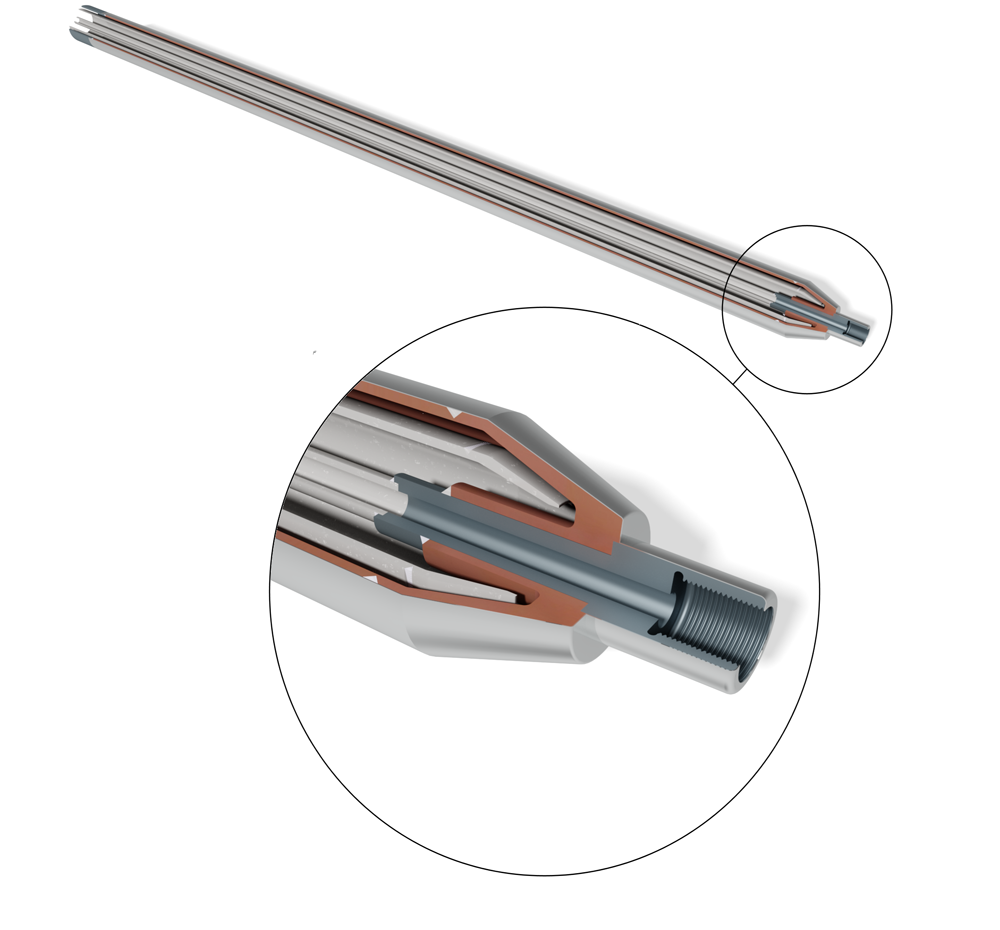
\includegraphics[width=6.5cm]{figures/sub-lance-berry.png} }}%
	\qquad
	\subfloat[Odber vzorky taveniny odbernou sondou v praxi.]{{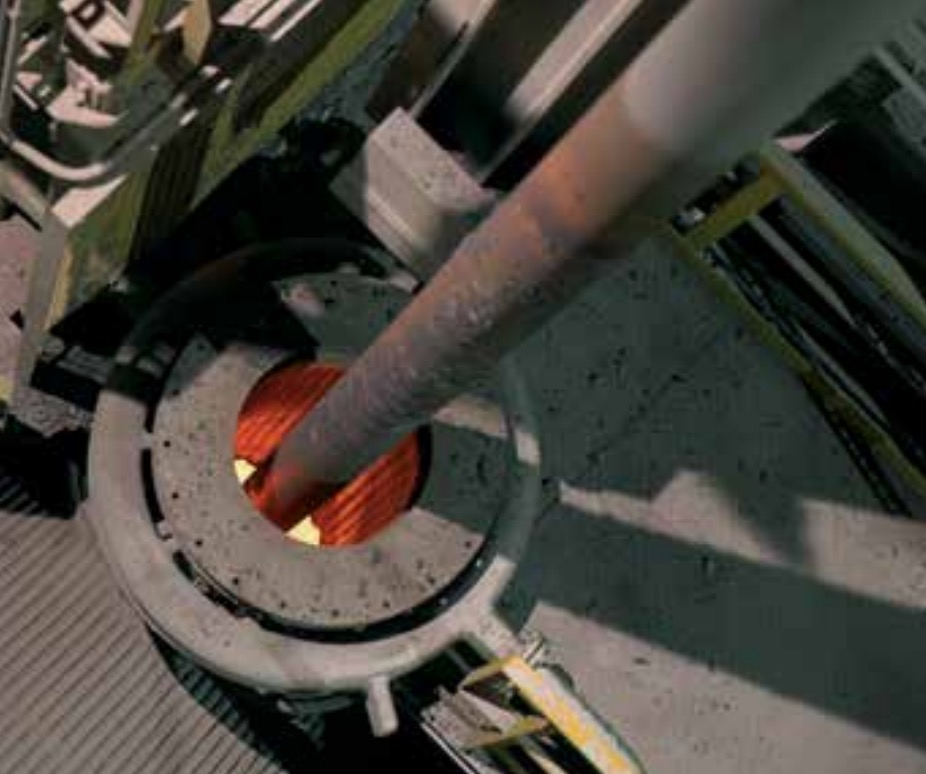
\includegraphics[width=7.35cm]{figures/sublance.jpg} }}
	\caption{Odberná sonda.}
\end{figure}

Moderné konvertory prevádzkujú merania odbernými sondami v spojení s kombinovaným statickým a dynamickým modelom riadenia procesu (SDM). Informácie získané z odbernej sondy sú ďalej spracované riadiacim systémom, ktorého optimalizačný model sa v konečnom dôsledku snaží o zvýšenie produkcie a dosiahnutie požadovaných vlastností ocele.

\section{Spracovanie dát}

\section{Uchovanie dát}


\section{Komunikačné protokoly}

OPC - Object Linking and Embedding for Process Control

priemyselné konzorcium OPC Foundation vytvára a udržiava viacero štandardov pre otvorené pripojenie zariadení a systémov priemyselnej automatizácie, ako sú priemyselné riadiace systémy a riadenie procesov všeobecne

\subsection{OPC UA}
 %OPC Unified Architecture (OPC UA) is a vendor-independent communication protocol for industrial automation applications. It is based on the client-server principle and allows seamless communication from the individual sensors and actuators up to the ERP system or the cloud. The protocol is platform-independent and features built-in safety mechanisms. Since OPC UA is flexible and completely independent, it is regarded as the ideal communication protocol for the implementation of Industry 4.0.
 

OPC Unified Architecture (OPC UA) je komunikačný protokol nezávislý od dodávateľa pre aplikácie priemyselnej automatizácie. Je založený na princípe klient-server a umožňuje plynulú komunikáciu z jednotlivých senzorov a akčných členov až do ERP systému alebo cloudu. Protokol je nezávislý od platformy a má zabudované bezpečnostné mechanizmy. Pretože OPC UA je flexibilný a úplne nezávislý, považuje sa za ideálny komunikačný protokol pre implementáciu Industry 4.0.

\begin{figure}[h!]
	\centering
	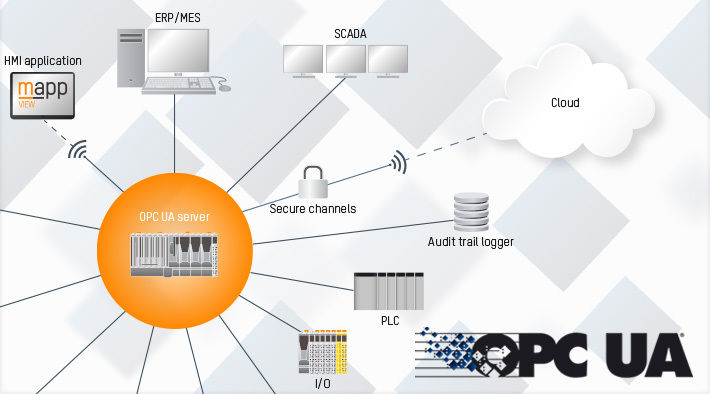
\includegraphics[width=.9\textwidth,angle=0]{figures/opc-ua.jpg}
	\caption{Grafická reprezentácia architektúry komunikačného protokolu OPC UA, zdroj: B\&R Automation.}
\end{figure}

%OPC UA bridges the gap between the IP-based world of IT and the production floor. Interfaces, gateways and the associated loss of information are a thing of the past because all production process data is transferred via a single protocol – within a machine, between machines or between a machine and a cloud database. OPC UA is eliminating the need for traditional factory-level fieldbus systems.

OPC UA premosťuje priepasť medzi svetom IT založeným na IP a výrobnou úrovňou. Rozhrania, brány a súvisiaca strata informácií sú minulosťou, pretože všetky údaje o výrobných procesoch sa prenášajú prostredníctvom jediného protokolu - v stroji, medzi strojmi alebo medzi strojom a databázou cloud. OPC UA eliminuje potrebu tradičných systémov priemyselnej zbernice na úrovni výroby \citep{brautomation}.

%When it comes to complex applications like safety, motion control and real-time communication, however, OPC UA has had its limitations. Since being expanded with the publish-subscribe model (pub/sub) and the Time-Sensitive Networking (TSN) Ethernet standard, OPC UA is now capable of real-time communication.

Pokiaľ ide o zložité aplikácie, ako sú bezpečnosť, riadenie pohybu a komunikácia v reálnom čase, OPC UA má však svoje obmedzenia. Od rozšírenia o model publikovania a prihlásenia na odber (pub / sub) a štandardu Ethernet citlivého na čas (TSN) je OPC UA teraz schopná komunikovať v reálnom čase.

\begin{figure}[h!]
	\centering
	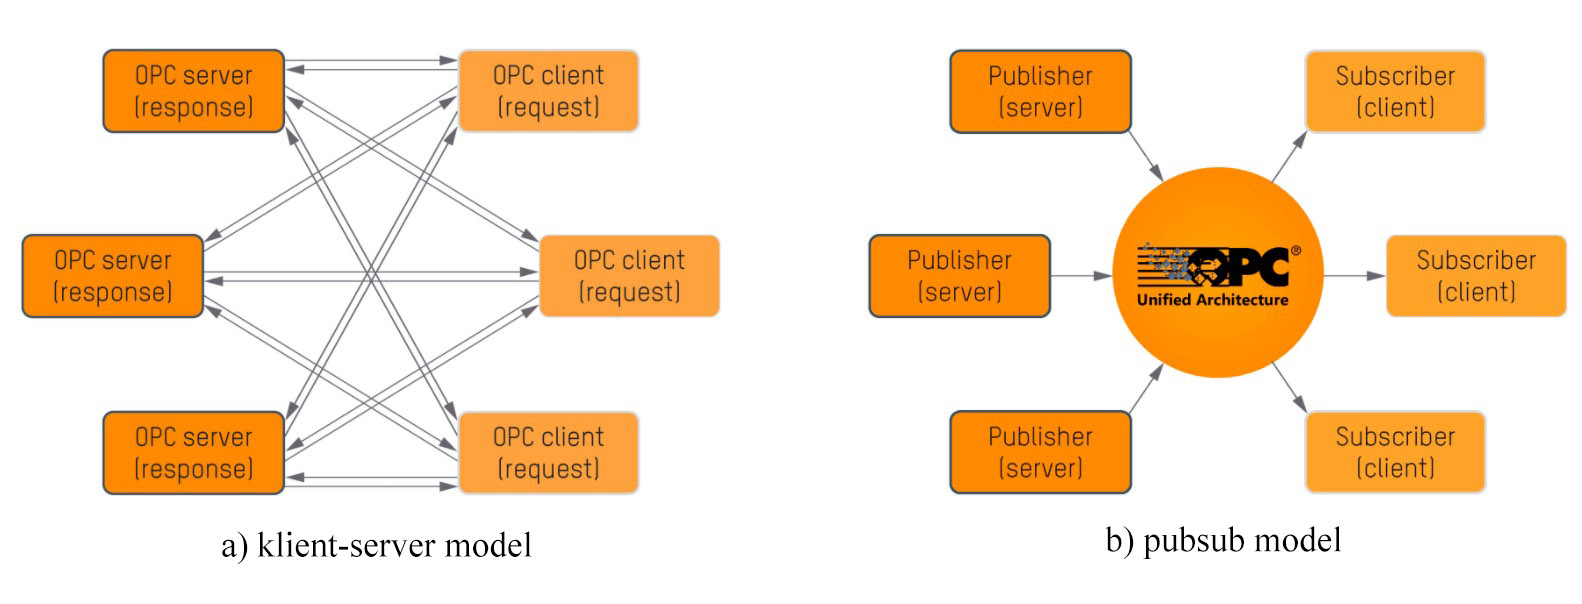
\includegraphics[width=1\textwidth,angle=0]{figures/opc-ua-pubsub.jpg}
	\caption{Rozdiel medzi architektúrou klient/server a publish/subscribe (počúvanie zmien po ju), zdroj: B\&R Automation.}
\end{figure}

\subsection{MTConnect}

Priemyselné systémy tvorí množstvo zariadení, často od rôznych výrobcov s rôznymi konkurenčnými výhodami. Od integrácie hardvéru do uceleného riešenia výrobných systémov vo výrobných podnikoch je v súčasnosti neoddeliteľná aj časť implementácie softvérovej nadstavby. Práve schopnosť adaptovateľnosti softvéru ako informačného systému pre podporu riadenia výrobných procesov podniku udáva, do akej miery je možné architektúru systému škálovať. Táto schopnosť v priemysle závisí vo vysokej miere na štandardoch. Súčasne dostupné softvérové riešenie preto využívajú štandardizáciu údajov a dát zo zariadení, pričom počítajú s tým, že každý výrobca môže označovať tieto dáta inak.

Norma MTConnect (ANSI/MTC1.4-2018) štandardizuje údaje a dáta výrobných zariadení naprieč rôznymi výrobcami. Ponúka sémantickú slovnú zásobu pre výrobné zariadenia na poskytovanie štruktúrovaných, kontextualizovaných údajov bez proprietárneho formátu.

\begin{figure}[h!]
	\centering
	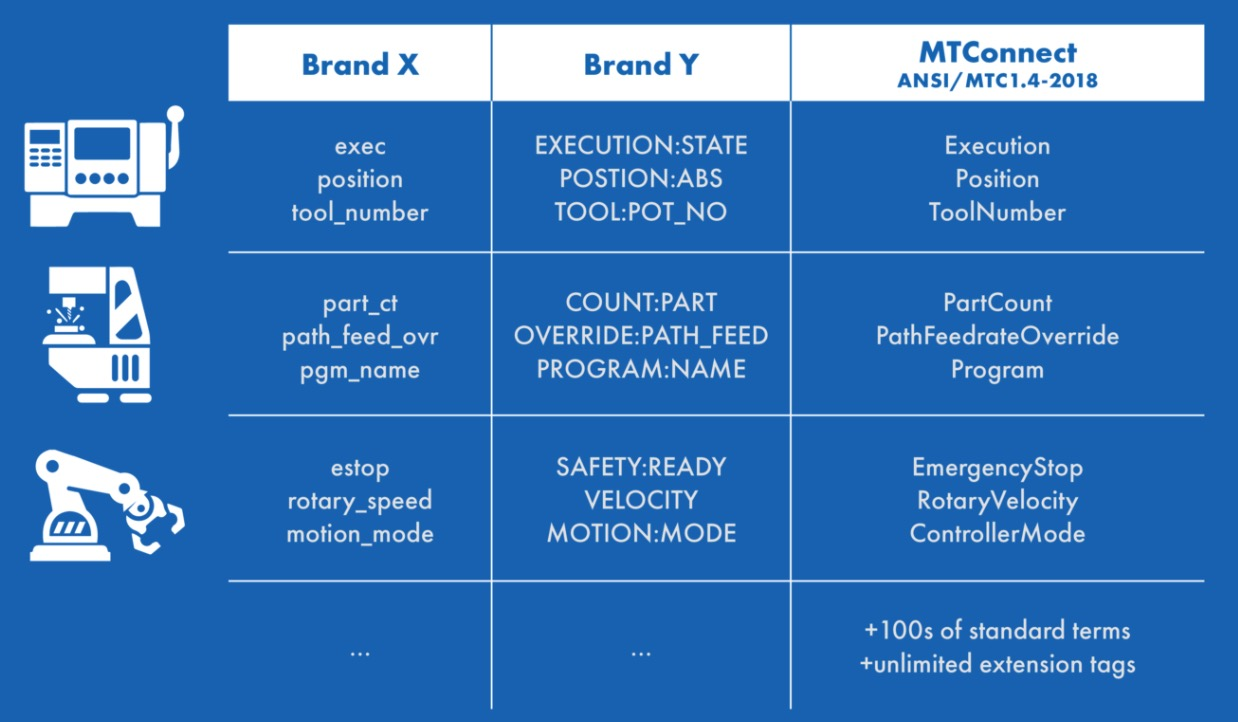
\includegraphics[width=.8\textwidth,angle=0]{figures/mtconnect.jpg}
	\caption{Tabuľka s ukážkou sémantickej výbavy normy MTConnect, zdroj: mtconnect.org.}
\end{figure}

MTConnect poskytuje doménovo-špecifickú slovnú zásobu a dátové modely, je rozšíriteľný a je ho možné kombinovať s inými štandardmi. Vďaka jednotným údajom sa vývojári a integrátori môžu sústrediť skôr na užitočné produktívne výrobné aplikácie než na preklady premenných. MTConnect ale nie je softvér; je to štandard, ktorý definuje dátové štítky a správanie sa softvérového agenta (časti informačného systému pre správu dát). Zdroje údajov zahŕňajú obrábacie stroje, výrobné zariadenia, senzory s ich ovládačmi a ďalší hardvér výrobcu. Aplikácie, ktoré spotrebúvajú údaje MTConnect, poskytujú efektívnejšie operácie a zlepšenú optimalizáciu výroby, čoho výsledkom je zvýšenie produktivity.

Za viac ako 10 rokov od prvého vydania tejto normy sa jej používanie rozšírilo na viac ako 50 000 zariadení od vyše 300 výrobcov vo viac ako 50 krajinách; existuje cez 1000 softvérových riešení implementujúcich túto normu.

\subsection{OMG DDS}

Služba distribúcie údajov (DDS) je middlewarový protokol a štandard API pre konektivitu zameranú na údaje z Object Management Group (OMG). Integruje komponenty systému dohromady a poskytuje dátové pripojenie s nízkou latenciou, extrémnu spoľahlivosť a škálovateľnú architektúru, ktorú potrebujú obchodné a kritické aplikácie internetu vecí (IoT).

V distribuovanom systéme je middleware softvérová vrstva, ktorá leží medzi operačným systémom a aplikáciami. Umožňuje rôznym komponentom systému ľahšiu komunikáciu a zdieľanie údajov. Zjednodušuje sa vývoj distribuovaných systémov tým, že sa vývojári softvéru môžu zamerať skôr na konkrétny účel svojich aplikácií než na mechaniku prenosu informácií medzi aplikáciami a systémami \citep{ddsfoundation}.

\section{Vizualizácia dát}


\section{Virtuálna realita}





\section{Procesy v kyslíkovom konvertore}

Kyslíkový konvertor alebo v niektorých oblastiach sveta nazývaný aj základná kyslíková pec (basic oxygen furnace - BOF) pozostáva z radu komplexných procesov s nebezpečnými vlastnosťami, napríklad z dôvodu vysokej teploty, prachu a vibrácií. V konvertore prebieha  množstvo chemických reakcií a fyzikálnych javov, medzi ktorými sa nájdu aj také, ktorým úplne nerozumieme z dôvodu ich komplexnosti.

Podstatou výroby ocele v kyslíkovom konvertore je oxidácia prvkov z kovonosnej vsádzky s kyslíkom fúkaným do konvertora. Oxidy týchto prvkov prechádzajú do trosky alebo odchádzajú vo forme konvertorového plynu. LD proces sa skladá z~nasledujúcich elementárnych procesov:

\begin{enumerate}
	\item Vsádzanie šrotu
	\item Nalievanie tekutého surového železa
	\item Fúkanie kyslíka a pridávanie troskotvorných a legujúcich prísad
	\item Meranie teploty a zloženia ocele
	\item Odpich ocele
	\item Odpich trosky
\end{enumerate}

V moderných oceliarňach sa vyrobí cca 300t ocele v priebehu 30-40 minútového cyklu. Pre prispôsobenie akosti ocele a tvorbu trosky sa počas pochodu pridávajú rozličné prísady. Počas vsádzania a odpichu je konvertorová pec naklonená. Počas fúkania kyslíka má konvertor zvislú polohu.

V závislosti od miestnych prevádzkových podmienok, dostupnosti šrotu, vysokopecného železa a rozsahu predúpravy, je kovová vsádzka do konvertora (LD/BOF, Q-BOP) tvorená 75 až 95 \% surovým železom a zvyšok je oceľový šrot. Používané druhy šrotu sú zvyčajne tie, ktoré sa vyrábajú v oceliarni: šrot z plechu, poškodené formy, plechovky a podobne \cite{Turkdogan1996}.

Kyslík je fúkaný vysokou rýchlosťou (až do dvojnásobnej rýchlosti zvuku) na povrch kovového kúpeľa v konvertore a v oblasti povrchu sa vytvára tzv. horúce miesto, kde prúd kyslíka naráža na povrch. Oxidačné produkty sa rozpustia v troske s výnimkou oxidu uhoľnatého, ktorý prechádza vrstvou trosky a tvorí hlavnú zložku konvertovaného plynu. Intenzita oxidácie jednotlivých prvkov závisí od ich chemickej afinity ku kyslíku. Oxidácia uhlíka je jedným z najdôležitejších procesov.

\begin{figure}[h!]
	\centering
	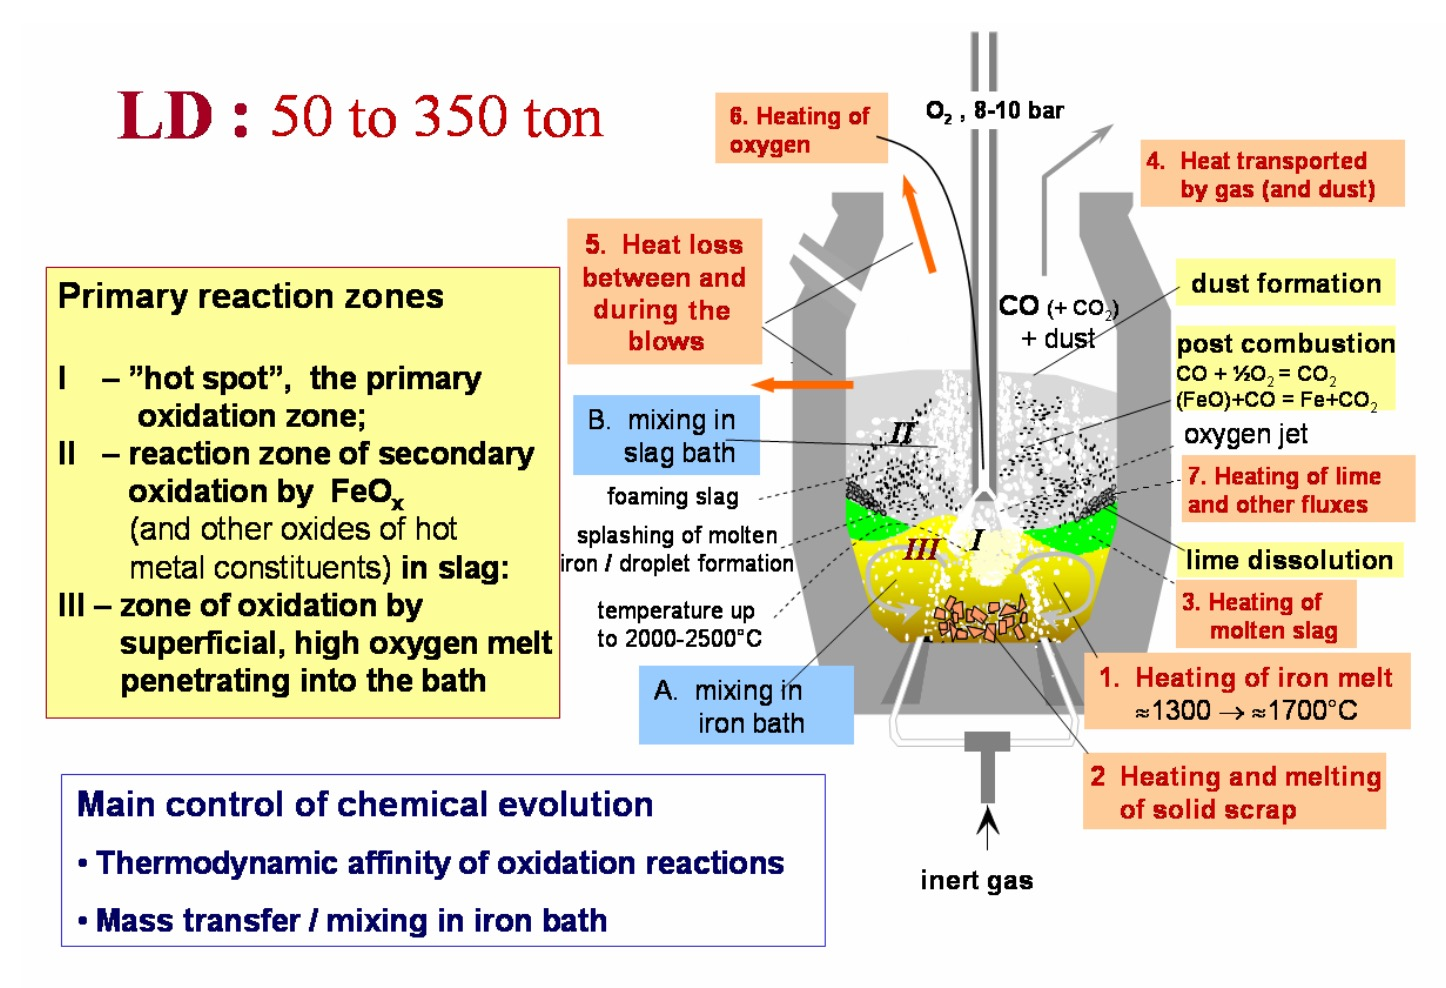
\includegraphics[width=1\textwidth,angle=0]{figures/ld-convertor-processes-graphical.jpg}
	\caption{Grafické znázornenie chemických a termodynamických procesov v LD konvertore \citep{Jalkanen2006}.}
\end{figure}

\section{Riadenie procesov v kyslíkovom konvertore}

Keďže cieľom výroby ocele v kyslíkových konvertoroch je spálenie (tzv. oxidácia) nežiadúcich nečistôt obsiahnutých v kovovej vsádzke, účelom tohto oxidačného procesu teda je:

\begin{itemize}
	\item znížiť obsah uhlíka na predpísanú úroveň (z približne 4 \% na menej ako 1 \%, ale často nižšie),
	\item upraviť obsah potrebných cudzích prvkov,
	\item odstrániť nežiadúce nečistoty v maximálne možnej miere.
\end{itemize}

Následnou úlohou riadiaceho procesu je potom získanie predpísaných parametrov ocele, ktorá sa odpichuje z konvertora, vrátane hmotnosti, teploty a obsahu každého prvku. Na základe týchto parametrov sa rozhoduje o tom, či je roztavená oceľ prijateľná alebo nie.

Počítačom podporované výpočty vsádzky sa robia pre každú tavbu. Asi 80 percent modelu riadenia vsádzky je založený na rovnováhe tepla a materiálu, zvyšok je založený na empirických vzťahoch, ktoré sa medzi jednotlivými taviarňami líšia. Pretože každá oceliareň má svoju vlastnú formuláciu modelu riadenia vsádzky \cite{Turkdogan1996}.



%
%%
\Urlmuskip=0mu plus 1mu\relax
\bibliographystyle{spbasic}
\bibliography{refs/control,refs/mathematics,refs/modeling,refs/cfd,refs/lbm,refs/gpu,refs/interaction,refs/interfaces,refs/hci,refs/design,refs/ml,refs/visualization,refs/programming,refs/simulation,refs/ar,refs/vr,refs/online}

%

\end{document}
%%